\documentclass[a4paper,12pt]{article}

\usepackage[final]{pdfpages}

\definecolor{clink}{rgb}{0,0,0.4}
\definecolor{ccite}{rgb}{0,0,0.4}
\usepackage[pdftex]{hyperref}
\hypersetup{colorlinks, backref, pdfpagemode=None, linkcolor=clink,
            citecolor=ccite, urlcolor=clink, pdfhighlight=/I, pdfstartview=FitH,
            pdfauthor=F.D.Bianchi, breaklinks}


\usepackage{databib}
\usepackage[
    backend=bibtex8, firstinits=true, style=authortitle, bibencoding=auto,
    maxnames=15, url=false, sorting=ynt, citereset=subsection,
    defernumbers=true]{biblatex}
\input{../biblatex_macros.tex}
\addbibresource{../../MyPublications.bib}
\setlength{\bibhang}{0.0cm}
\defbibheading{bibliography}{\large\bf This is a pre-print of the article:\vspace{1cm}}


\setlength{\parindent}{0.0cm}


\begin{document}


\thispagestyle{empty}

\vspace{3cm}

\nocite{Bianchi2004a}
\printbibliography

\vspace{3cm}
DOI: \href{https://doi.org/10.1016/j.renene.2004.02.009}{10.1016/j.renene.2004.02.009}

\vspace{1.5cm}
Url: \url{http://www.sciencedirect.com/science/article/pii/S0960148104000886}

\newpage
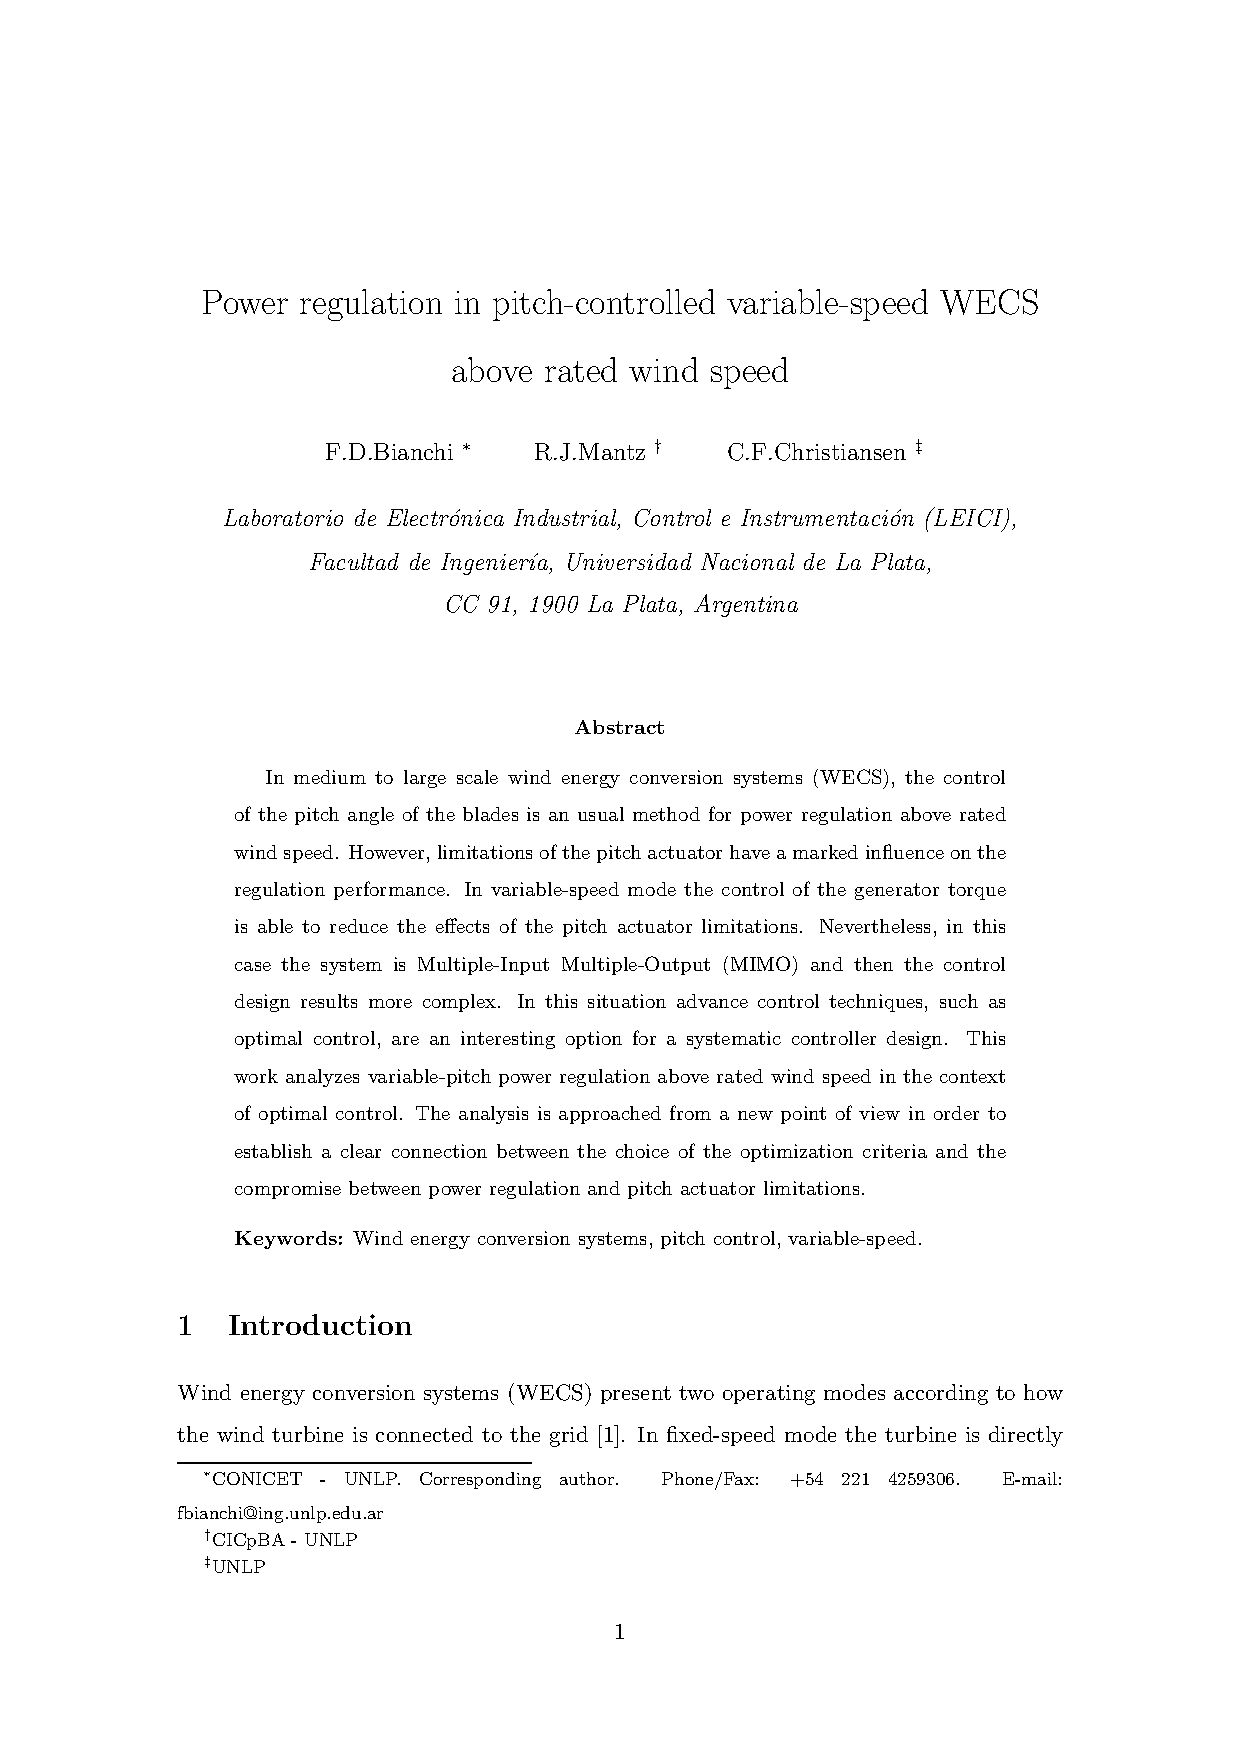
\includepdf[pages=-]{2004_RENE.pdf}



\end{document}

